%\documentclass[11pt, twoside, titlepage, a4paper, openright]{report}
\documentclass[12pt, oneside, titlepage, a4paper]{report}
\usepackage{graphicx}
\usepackage[english]{babel}
\usepackage[utf8]{inputenc}
\usepackage{algpseudocode}
\usepackage{amsthm}
\usepackage{algorithm}
\usepackage{rotating}
\usepackage{enumerate}
%\usepackage[Lenny]{fncychap}
\usepackage{hyperref}
\hypersetup{
    colorlinks=true,       % false: boxed links; true: colored links
    linkcolor=black,%red,          % color of internal links
    citecolor=black,%green,        % color of links to bibliography
    filecolor=black,%magenta,      % color of file links
    urlcolor=black%cyan           % color of external links
}
\usepackage [a4paper,left=2.5cm,bottom=2.5cm,right=2.5cm,top=3cm]{geometry}
\usepackage{frontespizio}

\newtheorem{mydef}{Definition} % definizioni <-----
%\nofiles 
%\fontoptionnormal 

\usepackage{mathtools}

\frenchspacing

\begin{document}


\begin{frontespizio}
\Universita {Verona}
\Dipartimento {Informatica}
\Corso {Ingegneria e Scienze Informatiche}
\Annoaccademico {2017-2018}
\Titoletto {Tesi di Laurea Magistrale}
\Titolo { \Large {Multi-Robot Task Allocation for logistic applications} }
\Candidato [vr414572]{Davide Zorzi}
\Relatore {Alessandro Farinelli}
\Correlatore{Riccardo Muradore}
\Rientro {1.5cm}
\NCandidato {Candidato}
\end{frontespizio}

%\clearpage\null\thispagestyle{plain}\clearpage
%\newpage

%\preparefrontpage

\tableofcontents

\newpage

\paragraph{Abstract}
\begin*{}
\newline
\newline
Robotics technology has recently matured sufficiently to deploy autonomous
robotic systems for daily use in several applications: from disaster response
to environmental monitoring and logistics.
In this project present and evaluate the principal difference of central and 
distributed allocator task coordinator. 
In these applications we address off-line coordination, by casting the Multi-Robot
logistics problem as a task assignment problem and proposing two solution 
techniques: Cyclic Greedy Strategy Single Robot Single Task (CGS1:1), which is 
a baseline greedy approach, and Cyclic Greedy Strategy Single Robot Multiple Task 
(CGS1:N), which is based on merging task for improve the spend time.
\\
And the last one is address on-line coordiantor, that is based on token passing (TP) approach.
We evaluate the performance of our system in a realistic simulation enviroment
(build with ROS and stage). In particular, in the simulated enviroment we compare
our task assignment approaches with previous off-line and on-line methods.
\newline
\newline
\textbf{Keywords:} Multi-Robot Task Allocator, logistic applications, Multi-Robot
systems, coordination, task assignment

% TODO: primi risultati e considierazioni

\end*{}




\chapter{Introduction}\label{chap:intro}

    \begin{frame}[fragile]{Industrial Logistics}
        The {\bf industrial logistics} is the process of {\bf planning}, {\bf organization}
        and {\bf control} of all the activities of handling and {\bf storage} of goods, which, starting
        from the suppliers and reaching up to the end user, guarantee an adequate
        level of {\bf service} to the customer consistent with the {\bf costs} to it associated

        \begin{figure}[hbt]
            \centering
            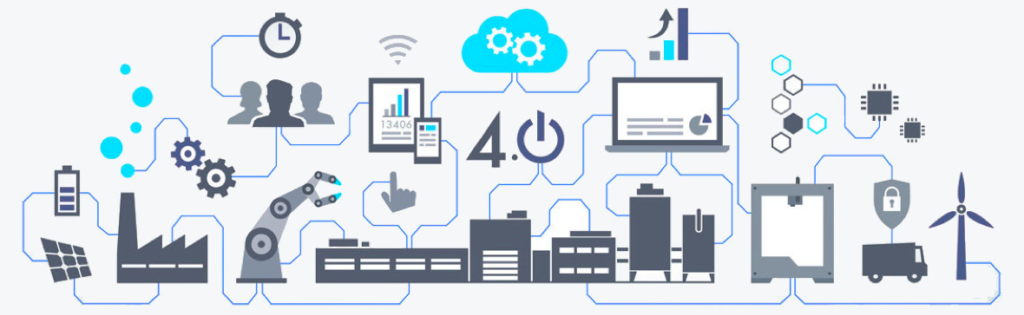
\includegraphics[width=\textwidth]{img/ind4.png}
        \end{figure}
    \end{frame}

    \begin{frame}[fragile]{Multi-Robot Systems for logistic applications}

        \begin{figure}[hbt]
            \centering
            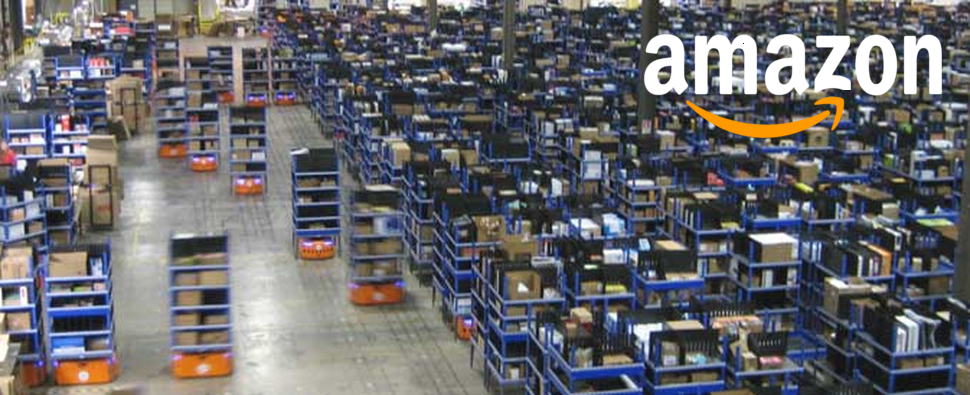
\includegraphics[width=\textwidth]{img/kiva.png}
        \end{figure}
        
        \begin{center}
        Kiva warehouse-management system
        \end{center}
    \end{frame}

    \begin{frame}[fragile]{Thesis contribution}
        \begin{center}
        The contribution of this thesis:
        \end{center}
        \begin{columns}
            \begin{column}{.7\textwidth}
           
            \begin{itemize}
            \item extension of  \texttt{ROS}  package
            \item proposing three tequnique:
            \begin{enumerate}
                \item Single robot : Single task (SR:ST) 
                \item Set Partition Strategy - Single robot : Multiple task (SPS1:N)
                \item Greedy Set Partition Strategy - Single robot : Multiple task (GSP1:N)
            \end{enumerate}
                \item real scenario: Computer Engineering for Industry 4.0 Laboratory (ICE Lab) 
            \end{itemize}
            \end{column}
            \begin{column}{.4\textwidth}
            \begin{figure}
                \subfloat{
\includegraphics[scale=0.45]{img/ros}}\qquad
                \subfloat{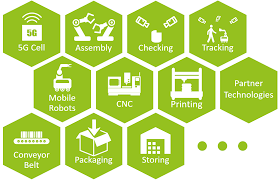
\includegraphics[scale=0.45]{img/ice}}
            \end{figure}
            \end{column}
        \end{columns}
    \end{frame}


    \begin{frame}[fragile]{ICE Laboratory}
        \begin{figure}[hbt]
            \centering
            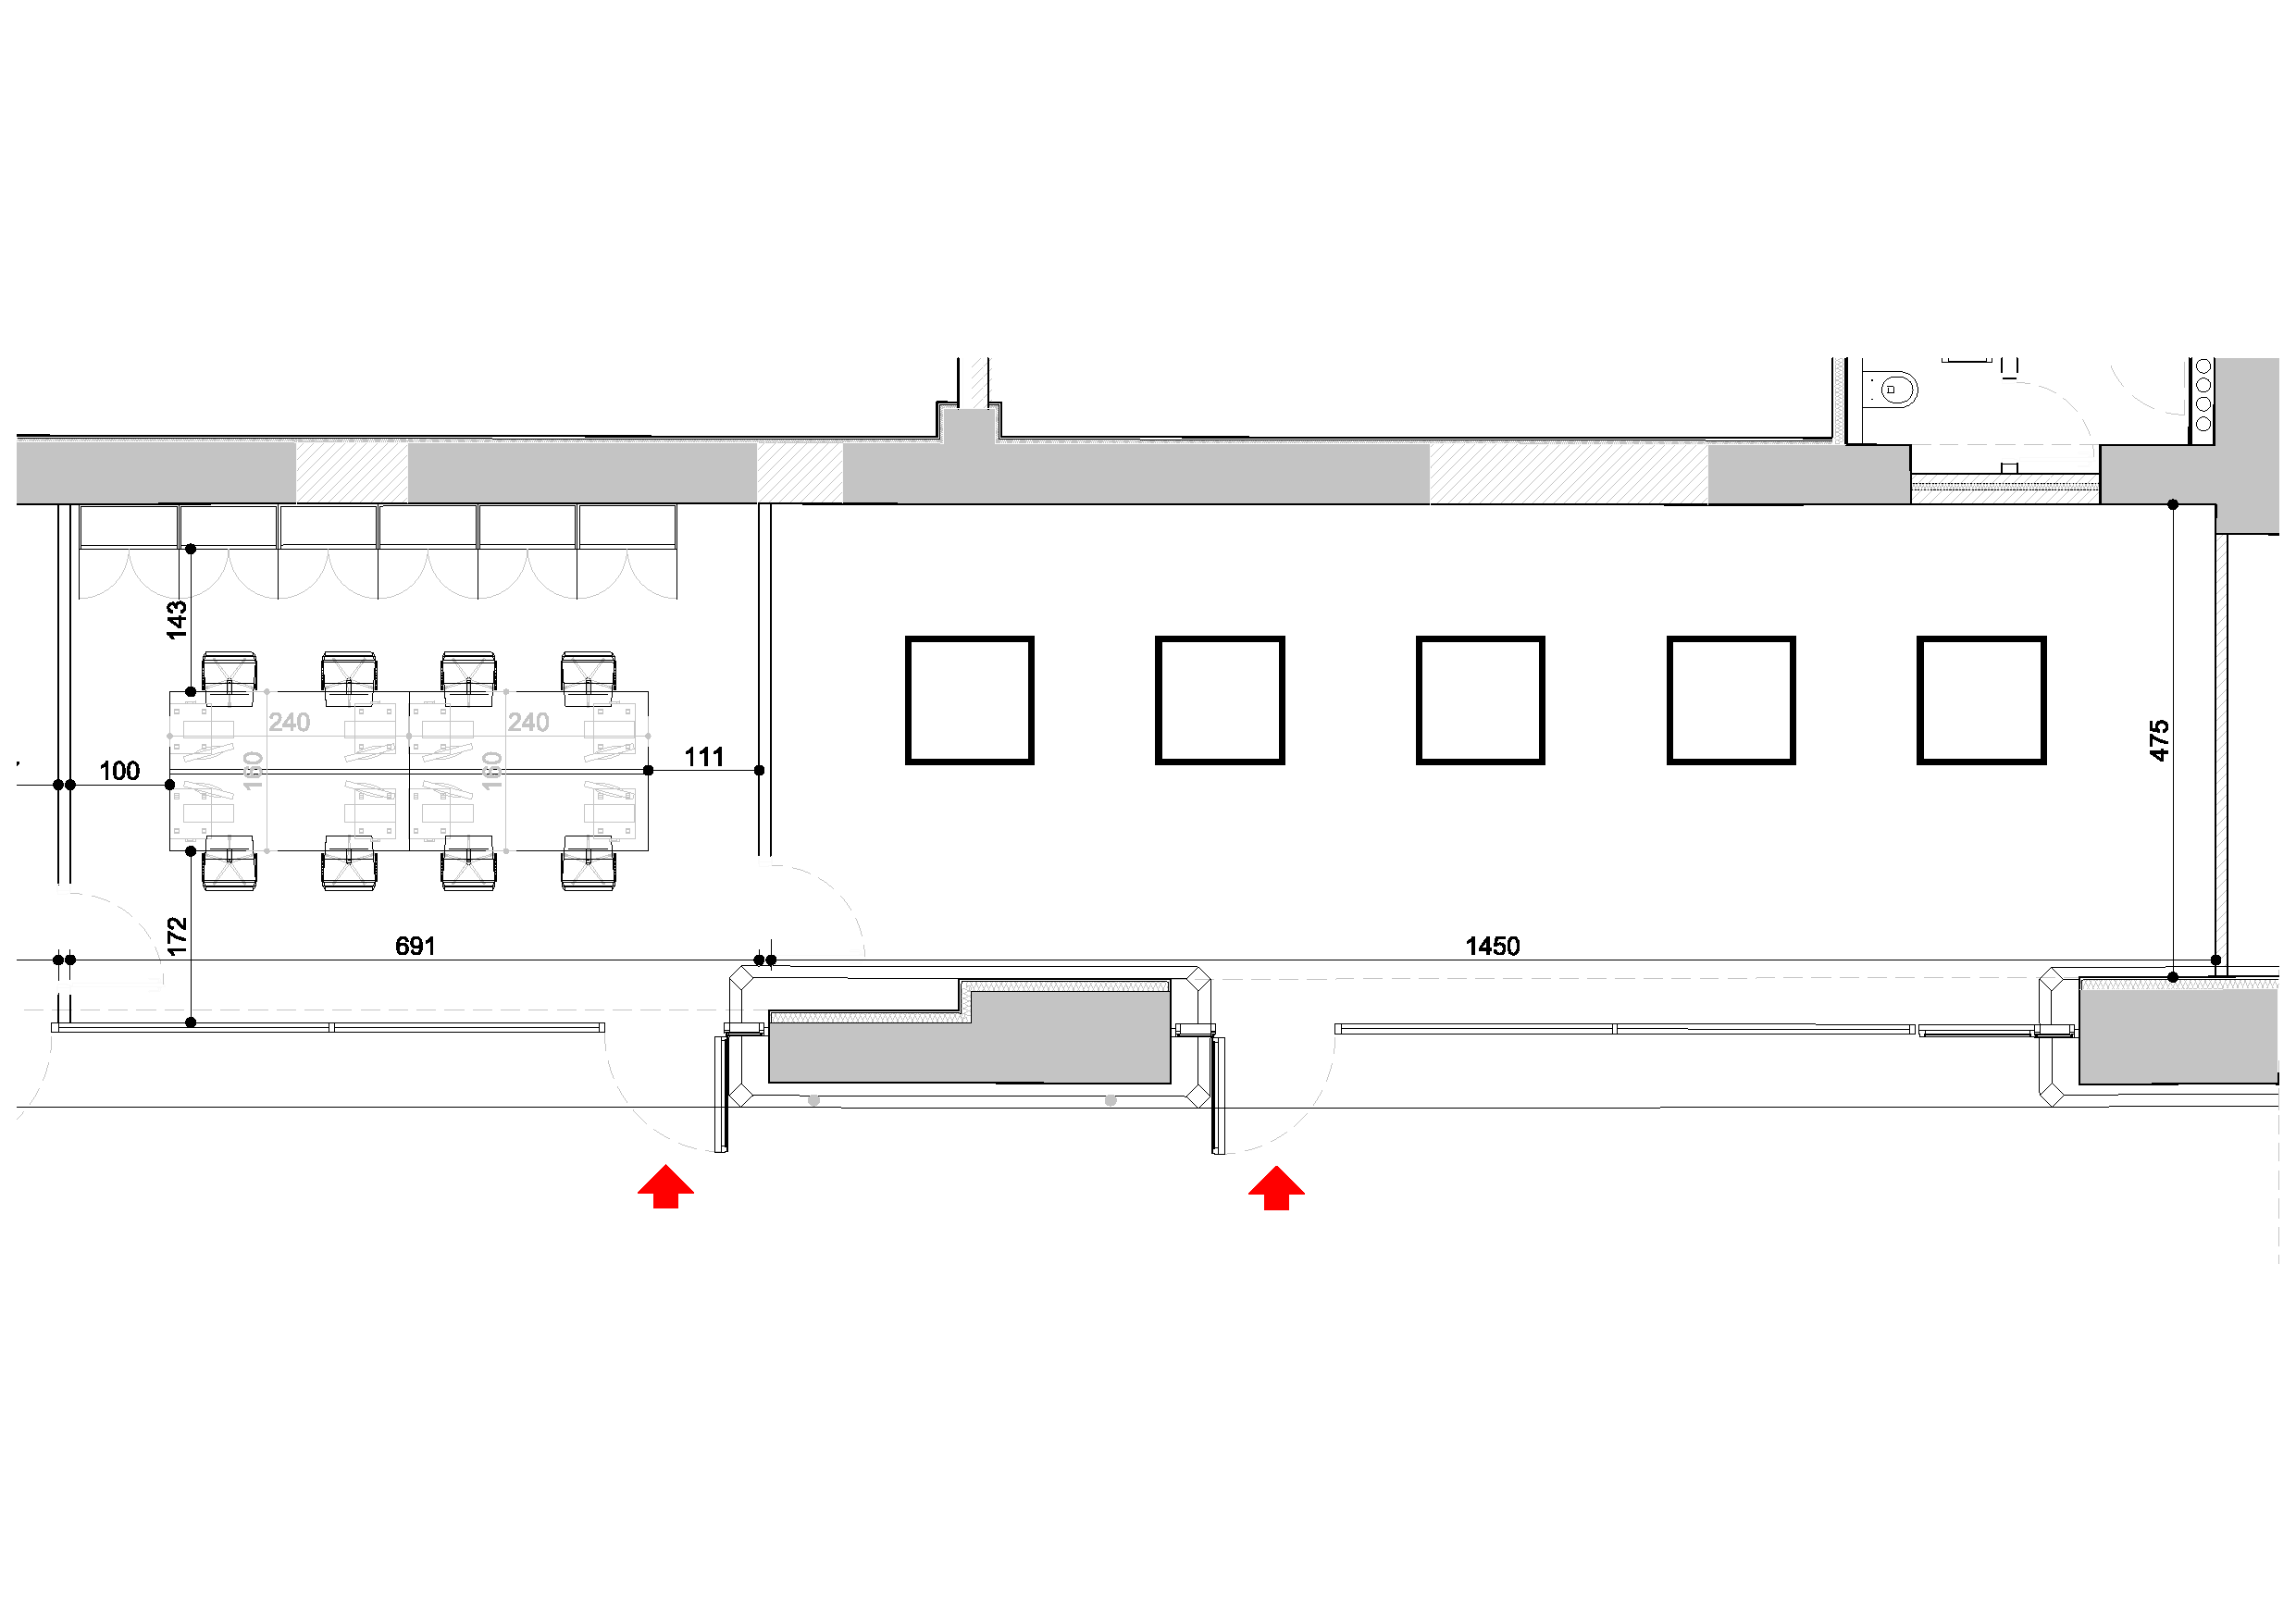
\includegraphics[width=\textwidth]{img/model1}
        \end{figure}
    \end{frame}

    \begin{frame}[fragile]{ICE Laboratory for logistic application}
        \begin{figure}[hbt]
            \centering
            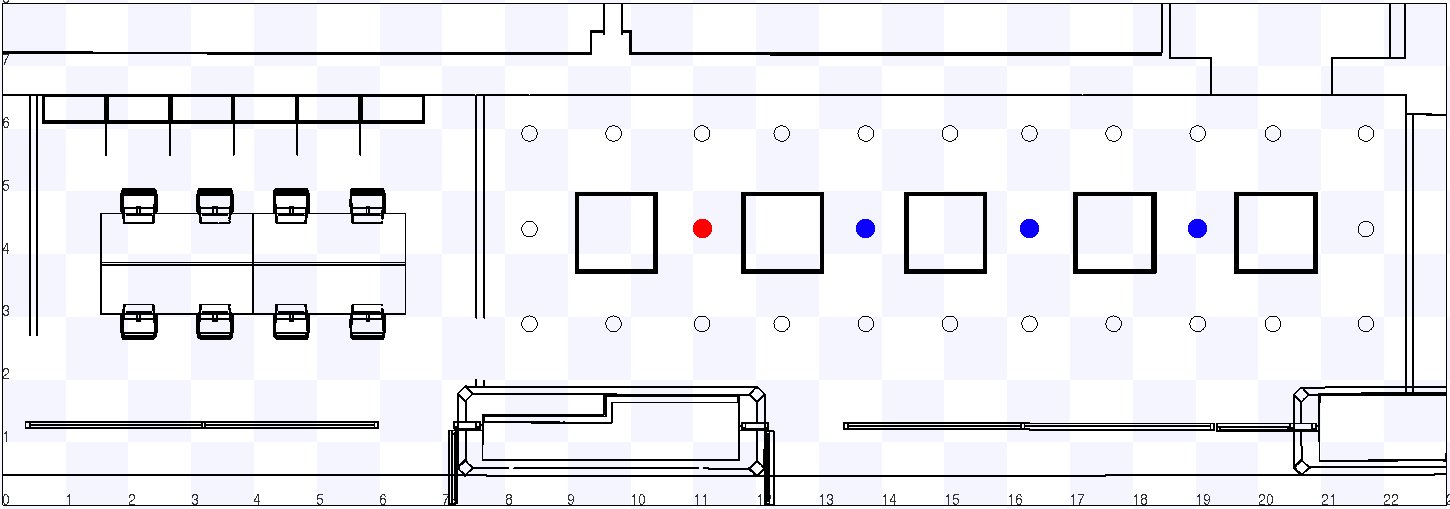
\includegraphics[width=\textwidth]{img/labgrafo}
        \end{figure}

        {\color{red}{$\bullet$}}  Loading bay
        \\
        {\color{blue}{$\bullet$}}  Unloading bays
        \\
        {\color{black}{$\circ$}}  Vertices
    \end{frame}

    \begin{frame}[fragile]{Set Partition Strategy - Single robot : Multiple task (SPS1:N)}
         \begin{columns}
            \begin{column}{.7\textwidth}
                \begin{center}
                    \begin{tabular}{|c|r|c|} \hline
                    \textbf{iteration} & \textbf{partition size} & \textbf{partition} \\ \hline
                    1    & 1    & \{\{a, b, c, d\}\}   \\
                    2    & 2    & \{\{a, b, c\}, \{d\}\}   \\
                    3    & 2    & \{\{a, b, d\}, \{c\}\}   \\
                    4    & 2    & \{\{a, b\}, \{c, d\}\}   \\
                    5    & 3    & \{\{a, b\}, \{c\}, \{d\}\}   \\
                    6    & 2    & \{\{a, c, d\}, \{b\}\}   \\
                    7    & 2    & \{\{a, c\}, \{b, d\}\}   \\
                    8    & 3    & \{\{a, c\}, \{b\},\{d\}\}   \\
                    9    & 2    & \{\{a, d\}, \{b, c\}\}   \\
                    10   & 2    & \{\{a\}, \{b, c, d\}\}   \\
                    11   & 3    & \{\{a\}, \{b, c\}, \{d\}\}   \\
                    12   & 3    & \{\{a, d\}, \{b\}, \{c\}\}   \\
                    13   & 3    & \{\{a\}, \{b, d\}, \{c\}\}   \\
                    14   & 3    & \{\{a\}, \{b\}, \{c, d\}\}   \\
                    15   & 4    & \{\{a\}, \{b\}, \{c\},\{d\}\}   \\ \hline       
                    \end{tabular}
                  \end{center}
            \end{column}
            \begin{column}{.4\textwidth}
            \begin{figure}
                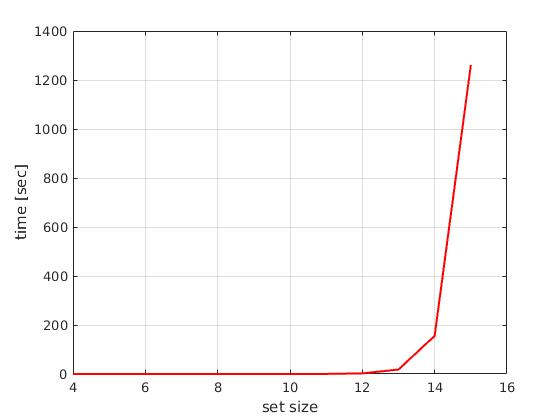
\includegraphics[width=\textwidth]{img/exp}
            \end{figure}
            \end{column}
        \end{columns}
    \end{frame}

    \begin{frame}[fragile]{Greedy Set Partition Strategy - Single robot : Multiple task (GSP1:N)}
    \end{frame}

    \begin{frame}[fragile]{ROS package Logistic\_sim}
        \begin{figure}[hbt]
            \centering
            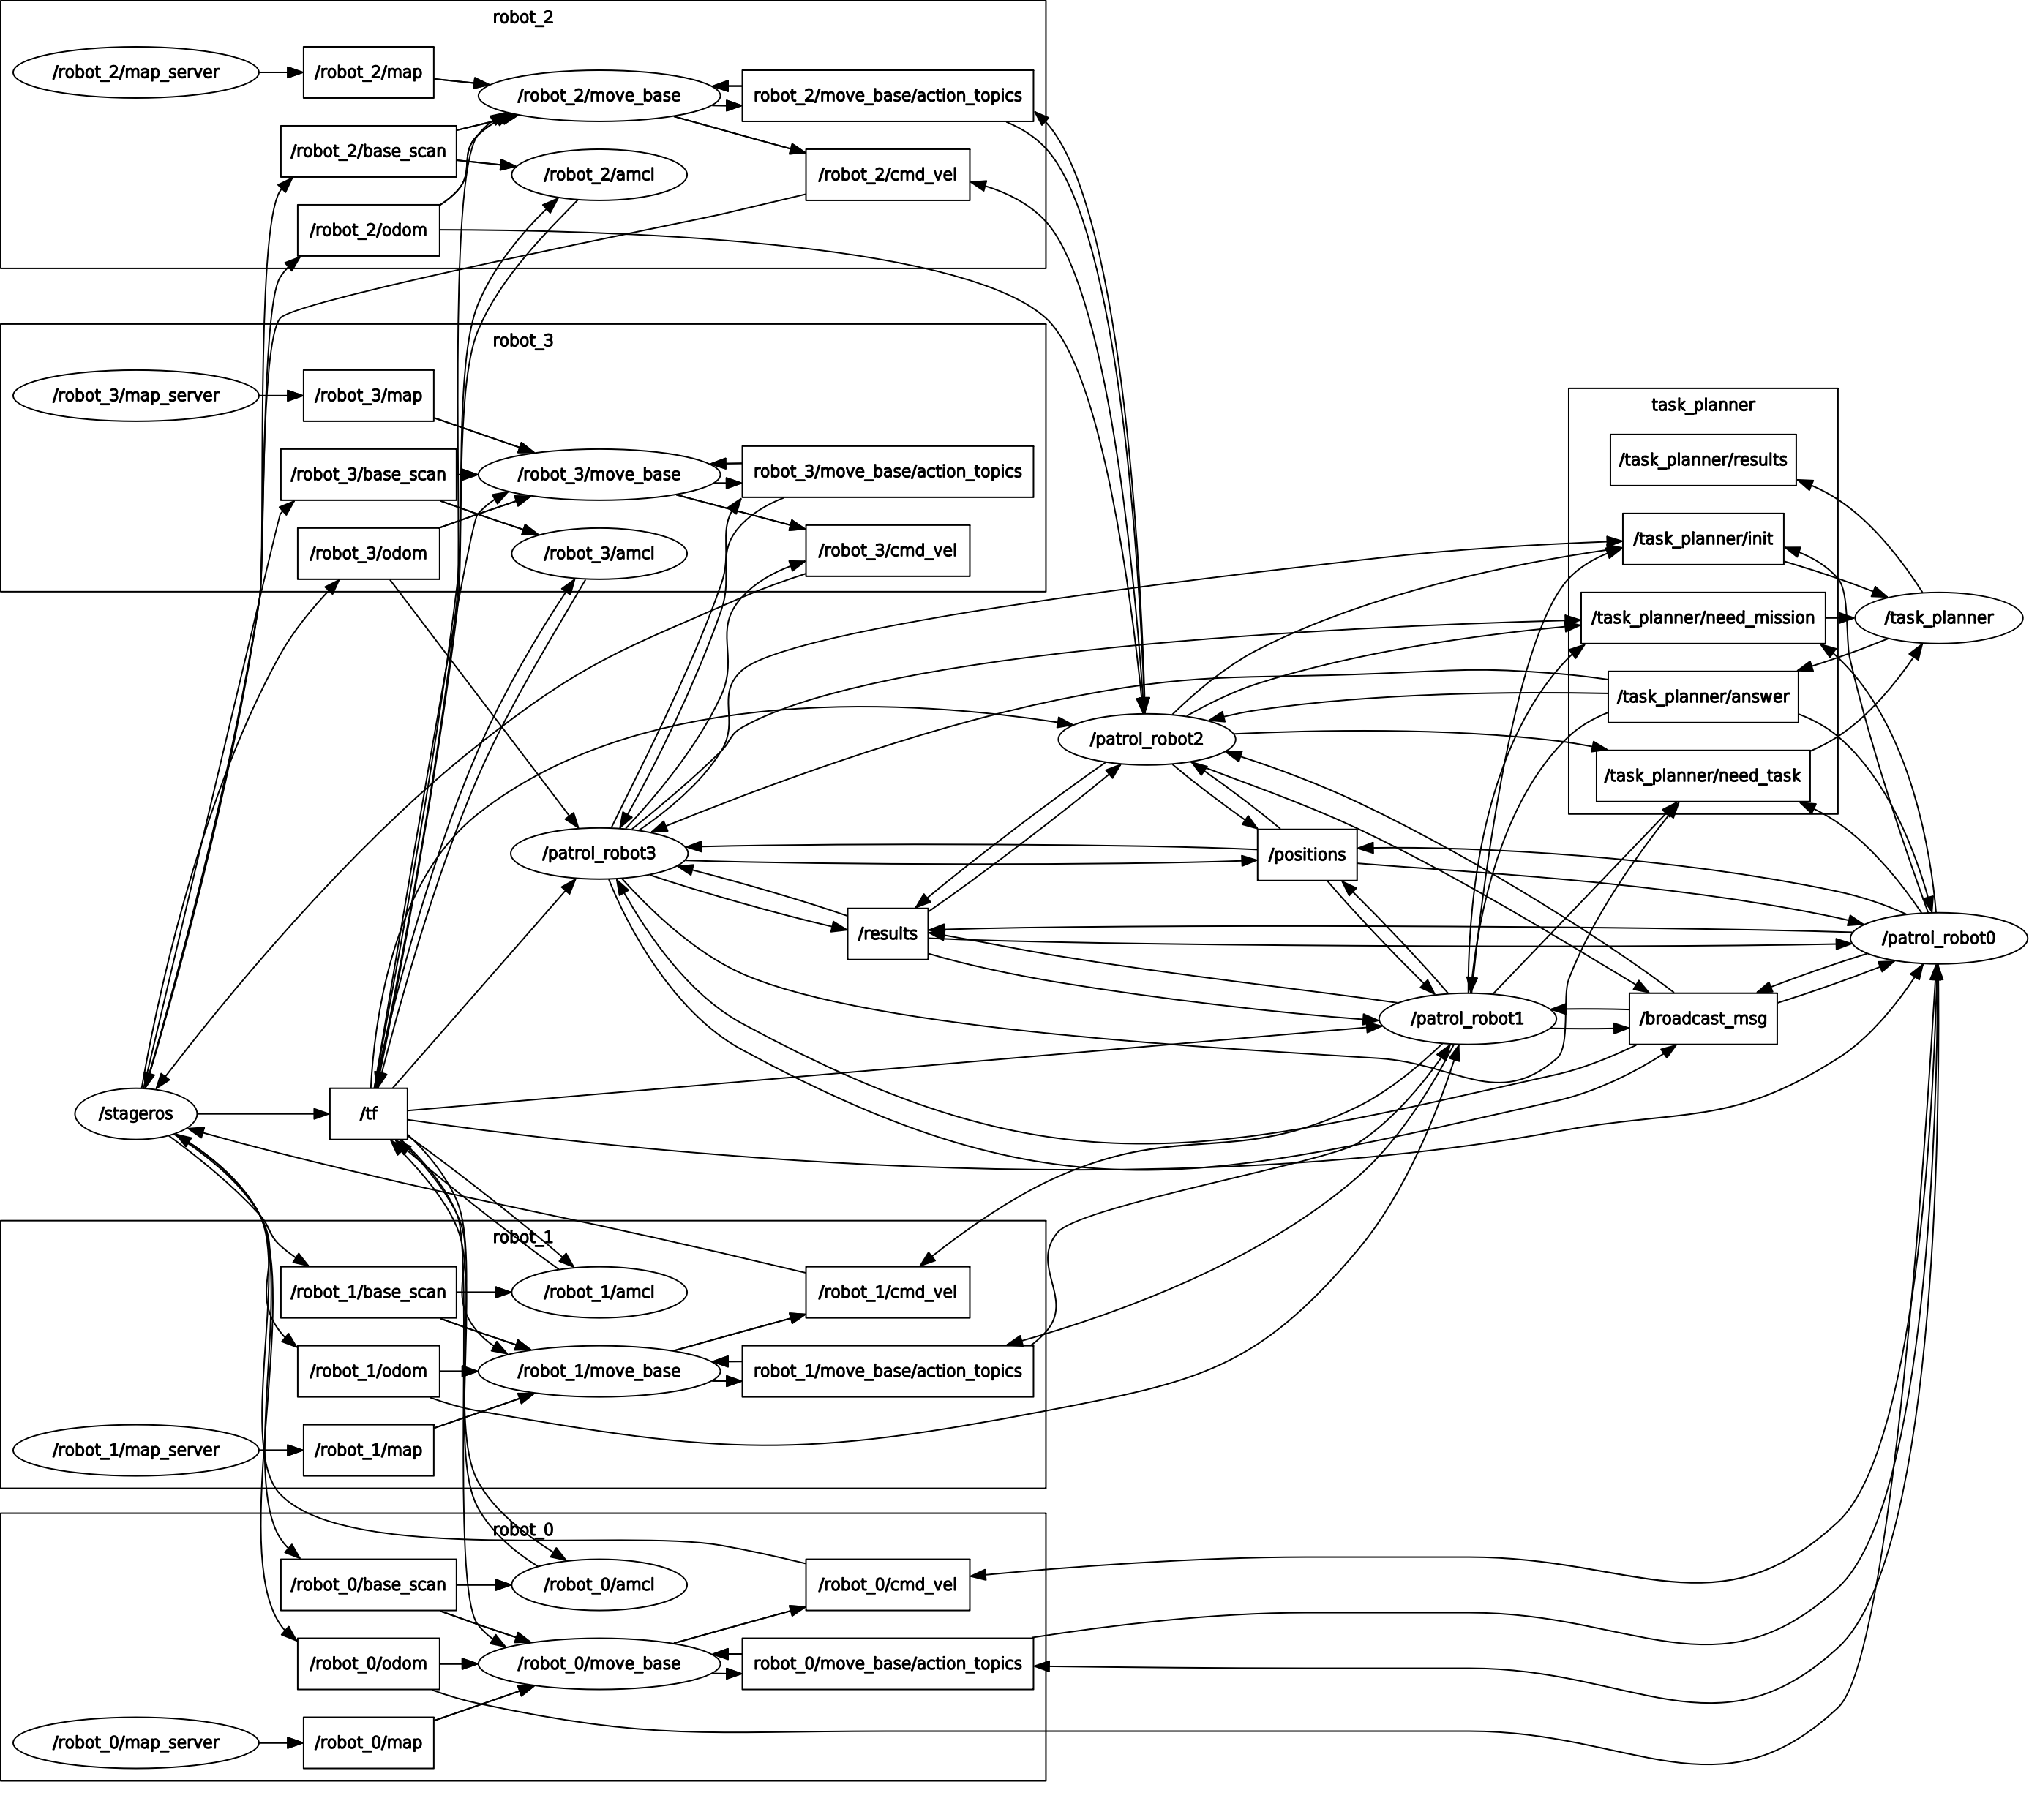
\includegraphics[scale=0.12]{img/rosgraph}
        \end{figure}
    \end{frame}

    \begin{frame}[fragile]{Empirical Results}
    \end{frame}

    \begin{frame}[fragile]{Video}
    \end{frame}

    \begin{frame}[fragile]{Conclusions and Future Work}
    \end{frame}









\chapter{Background and Related Works}\label{chap:related}
In this section, we detail the main issues for \mrs coordination 
in industrial domains, then we provide a detailed discussion on coordination
approaches, highlighting challenges and main solution techniques.

\section{Multi-Robot System for Industrial Applications}
In this thesis we also focus on industrial scenarios where robots have a high
degree of autonomy and operate in a dynamic environment.
\\
In article \cite{maxsum} robots must cooperate to maximizes the number of packages
completed in the unit of time. To this end a crucial component is to avoid interferences
when moving in the enviroment. They have formalised that problem as a Distributed 
Constrained Optimization problem based their solution on the binary max-sum algorithm.
\\
The most recent paper in logistic scenario \cite{mapd}, uses a Token Passing approach 
that solves the pickup-and-delivery tasks. The resulting algorithm takes kinematic 
constraints during planning, computes continuos agent movements with given velocities
that work on non-holonomic robots.

In this work, we consider a similar setting where a set of robots are involved
in trasportations tasks for logistics. However, we focus on the specific problem
of task assignment.

\section{Coordination in Multi-Robot system}
Coordination for \mrs has been investigated from several diverse
perspectives and nowadays, there is a wide range of techniques that can be used to 
orchestrate the actions and movements of robots operationg in the same enviroment.
Specifically, the ability to effectively coordinate the actions of a \mrs is a key 
requirement in several applications domains that range from disaster response to 
environmental monitoring, militaty operations, manufacturing and logistics. 
In all such domains, coordination has been addressed using various frameworks and 
techniques and there are several survery papers dedicated to categorize such different
approaches and identifying most prominent issues when developing \mrs.
\\
In the paper \cite{cooros} present and evaluate new ROS package for coordinated 
multi-robot exploration. The packages allow completely distributed control and do 
not rely on (but allow) central controllers.
\\
Given our focus on logistic scenarios, here we restrict our attention to coordination
approaches based on optimization and specifically on task assignment as this the most 
common framework for my reference application domain.

\chapter{Problem}\label{chap:problem}
In this section we detail our reference scenario for MRS coordination and as well 
as the formalization of the problem we addressed and the solutions we propose.

\section{Description}
Our reference scenario is based on a warehouse that stores items of various types.
Such items must be composed together to satisfy orders that arrive based on customers’ demand.
The items of various types are stored in particular sections of the building (\textit{loading bay})
and must be trasported to a set of \textit{unloading bays} where such items are then 
packed together by human operators. The set of items to be trasported and where they should
go depends on the orders.

In our domain a set of robots is responsible for transporting items from
the loading bays to the unloading bays and the system goal is to maximize the
throughput of the orders, i.e., to maximize the number of orders completed in
the unit of time. Now, robots involved in transportation tasks move around
the warehouse and are likely to interfere when they move in close proximity,
and this can become a major source of inefficiency (e.g., robots must slow down
and they might even collide causing serious delays in the system).

Hence, a crucial aspect to maintain highly efficient and safe operations is to minimize the
possible spatial interferences between robots.
%  dire che ci focaliziamo sull'unione di pezzi del path


\section{Fomalization}
In this section we formalize the MRS coordination problem described above as a task allocation problem
where the robots must be allocated to transportation tasks. 

In our formalization we have a finite set of task. A robot can execute a task if it is available else the robot will go at start position.
For how the system is built, a robot to request a task must arrive at the previous vertex of the loading bay.

In more detail, our model considers a set of items of different types $E = \{ e_1,...,e_N\}$,
stored in a specific loading bay ($L$). The warehouse must serve a set of orders 
$O=\{o_1,...,o_M\}$. Orders are processed in one or more than one of the unloading bays ($U_i$).
Each order is defined by a vector of demand for each item type (the number of required 
items to close the order). Hence, $o_j = < d_{1,j},...,d_{N,j}>$, where $d_{i,j}$ is the 
demand for order $j$ of items of type $i$. When an order is finished a new one arrives,
until the set of task is finished.
The orders induce a set of $N \times M$ trasportation tasks $T = {t_{i,j}}$, with 
$t_{i,j} = < d_{i,j}, dst_{i,j}, P_{i,j}>$, where $t_{i,j}$ defines the task of transporting 
$d_{i,j}$ items of type $i$ for order $o_j$ (hence to unloading bay $U_j$).
Each task has a destination bay for centralized coordination the $t_{i,j}$ has a set of edges
$P_{i,j}$ which respects the strategy used. 
We have a set of robot $R = \{r_1,...,r_K \}$ that can execute transportation tasks, where
each robot has a defined load capacity for each item type $C_k = <c_{1,k},...,c_{N,k}>$, 
hence $c_{i,k}$ is the load capacity of robot $k$ for items of type $i$.

We consider in our logistic scenario, homogenous robots, which have the same radius 
and the same capacity. Because often in the logistic environments robots are all 
equal. 





\chapter{Solution}\label{chap:solution}

\chapter{Experiments}\label{chap:experiments}

\chapter{Conclusions}\label{chap:conclusions}

\chapter*{Acknowledgements}
\addcontentsline{toc}{chapter}{\protect\numberline{}Acknowledgements}

%\bibliographystyle{splncs03}
%\bibliography{biblio}

\end{document}
